\section{Recrossing Effect}
\label{sec:recrossing}
%focus, schwerpunkt, emphasis

%In the last section, we have seen that the projected transfer operator of a Markov process respectively its matrix representation inherit some of the most important properties of the original process. Two further desirable properties would be the maintainance of Markovianity and a correct long-time description of the Markov State Model. We will examine these two issues in this section
%For instance, one further desirable property would be a commuting behaviour in/concerning propagation and projection of the process. That is, it should make no difference in which order these two operations are executed.
%That is, it should make no difference if we propagate a projected process or if we project a propagated %process.
%Unfortunately/but it will turn out that this is not the case.

%examine/introduce. crucial/main points/issues/subjects/topics of this thesis. This effect, occuring/appearing
In this section, we examine the so called recrossing effect which is one of the main topics of this thesis.
%\marginpar{relation/difference to iteration error}
%arising
This effect occurs when projecting a process onto a smaller state space and may spoil the Markov Property of the process. %\marginpar{measure by $S$?}
%\marginpar{kind of memory effect}

We describe it by means of an easy example. %analyze/describe
%projected process/transfer operator. behaves/propagates
Additionally, we have to face the problem that a projected transfer operator does \textbf{not} necessarily propagates as the original process. We explain the relevance of this iteration error without going into further details, since in the following chapters we will be able to employ a projection where this error vanishes. %error/deviation
%construct/apply/use/employ a projection
%without going into further/deeper details/focus/emphasis,
%perform/execute/apply

%Furthermore, we will see the relation between the matrix representation from theorem \ref{thm:galerkin} %on the rebinding effect and how this effect can be measured considering the matrices $S$ and $T$.
%We will also compute some error estimations/bounds for the recrossing effect.

%In MD, the recrossing effect is also called \textit{rebinding effect}. Since the examination of the rebinding %effect is one of the main objectives of this thesis, we will put much emphasis on the mathematical %description of this effect.

%Now what is the stochastic interpretation of theorem \ref{thm:galerkin}? Can we get some insight into the %nature of $G \Pcal G$? $T$ is a transition matrix? Its Markovianity is spoiled by $S$? The closer $S$ is to the %unit matrix, the smaller the Recrossing effect?
%It will be examined later in section 2.4 after we examined the so called Recrossing effect which describes %the loss of Markovianity by projecting the process/ transfer operator. By $S$ and $T$, the recrossing effect %can be measured.

\subsubsection*{Initial Situation}

Assume we are given a Markov process $\markov$ on a continuous or very large state space $E$, described by the transfer operator $\Pcal := \Pcal(\tau)$.
% discretize the time
In order to get a discrete process out of it, we project the time onto $\mathbb{N}$ and the state space onto a finite set $\{1,\dots,n\}$.
%is easy/naturally
Discretizing the time can be done naturally without problems since for every lag-time $\tau > 0$, the process $(X_{k\tau})_{k\in \mathbb{N}}$ is again Markovian. \marginpar{why?}

%examined/observed
However, the state-space discretization has to be observed a bit more elaborated.
%Let's
We do this on the example of a full partition discretization.
% the (original) process
We consider the operator $G(\Pcal^k) := G\Pcal^k G$, that is we first propagate the process and project it afterwards.
%This is the ``correct projection''.
Then for all $k$-multiples of $\tau$, we assign the current state of the original process $X_t$ to the projected process $\widetilde{X}_k$:
\begin{equation*}
\widetilde{X}_k = i \Leftrightarrow X_{k\tau} \in A_i.
\end{equation*}
The process $\xtilde_k$ describes the \textit{snapshot dynamics} of $X_t$ with lag time $\tau$ between the partition sets $A_1,\dots,A_n$.
The so defined process is not necessarily Markovian, since $(G(\Pcal^k))_k$ is in general \textbf{not} a semigroup, [ ]. \marginpar{?}

\subsubsection*{Recrossing in a Double Well Potential}

%describing ... the motion of a particle?... in a double-well potential
Let $X_t$ be the Markov process corresponding to the double-well potential $V(x) = (x^2-1)^2$. We consider a full-partition of the state space into two sets $A$ and $B$ around the local minima of the energy landscape, as shown in figure \ref{fig:doublewell}.
We are interested if the induced process $\xtilde_k$ inherits the Markovianity of $X_t$ or if it contains any memory effects.
%contains/includes
\begin{figure}[!ht]
	\centering
	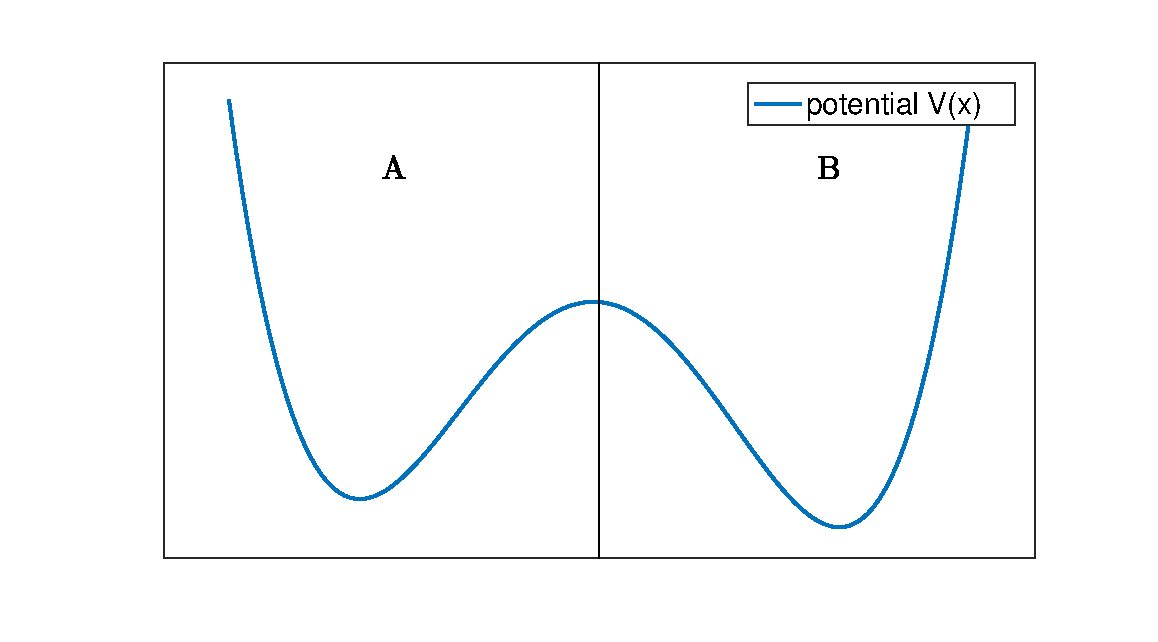
\includegraphics[width=0.6\textwidth]{figures/doublewell.eps} %70% der Textbreite
	\caption{Full-partition of a double-well potential}
	\label{fig:doublewell}
\end{figure}


For a small lag-time $\tau = 0.1$ we compute the probability of $\xtilde_k$ to make a transition from $B$ to $A$ in one time-step. We compare it to the probability of the same transition with the \textbf{additional} information of having been in $A$ one time-step before/earlier. If the process was Markovian, then this additional information about the past should make no difference and consequently, both probabilities should be equal.
We compute them in terms of the original process $X_t$ by
\begin{equation*}
\Prob_\mu[X_{(k+1)\tau} \in A \mid X_{k\tau} \in B] \textrm{ and }
\Prob_\mu[X_{(k+1)\tau} \in A \mid X_{k\tau} \in B, X_{(k-1)\tau} \in A].
\end{equation*}
Using the density functions $v_B$ and $v_{BA}$, we get %\marginpar{$v$ densities?}
\begin{equation}
\label{eq:recrossing1}
\Prob_\mu[X_{(k+1)\tau} \in A \mid X_{k\tau} \in B] = \int_A v_B^\tau(x) \diff x = ... ,
\end{equation}
\begin{equation}
\label{eq:recrossing2}
\Prob_\mu[X_{(k+1)\tau} \in A \mid X_{k\tau} \in B, X_{(k-1)\tau} \in A] = \int_A v_{BA}^\tau(x) \diff x = ... .
\end{equation}
We see that for such a short lag-time $\tau$, the process $\xtilde_k$ is \textbf{not} independent of the past  and hence \textbf{not} a Markov process.
%the process $\xtilde_k$ is \textbf{not} memoryless
%That behaviour is intuitively clear.
Equation \eqref{eq:recrossing1} describes the probability to get from $B$ to $A$, where ``being in $B$'' could mean everything from ``close to the transition region'' to ``far away from the transition region''. This probability is averaged over \textbf{all} possible starting points in $B$, since the spatial arrangement inside of $B$ is not included in this model. \marginpar{?} %specified/included
We compare it to \eqref{eq:recrossing2}, where being in $A$ shortly before
%immediately one time-step; moving to B
being in $B$ \textbf{increases} the probability to return to $A$ again. %return/recross
This behaviour can be interpreted such that for a short time after a \textbf{transition}, the process is likely to be still inside ot the \textbf{transition region}.
In our example, the transition region is the area close to the maximum of potential energy. Thus, there still is an increased probability to return to the previous state,
because of the spatial situation shortly after the transition. %area/region
\\

%transition between states = crossing the ``barrier'' between the states..

%the probability that the process is still in the transition region. And to get to $A$ from the transition region in $B$ is just more likely than from any other region inside $B$.
%favorable spatial situation?

This issue is called the \textit{recrossing effect}, since additional memory  leads to an increased probability to ``recross'' the energy barrier shortly after a transition. %(=energy maximum) %as in \eqref{eq:recrossing2}
On the other hand, if we choose a large lag-time, e.g. $\tau = 100$, then the past transition from $A$ to $B$ in \eqref{eq:recrossing2} took place a long time ago. In that case we do not know if the process is still in the critical transition region; during that long lag-time it could also have been gone anywhere else. %cannot certainly know
%That means that we could describe the memory effect of $\xtilde$ as a \textit{short-time memory}.
That means that the memory effect included in $\xtilde_k$ gets smaller for larger lag-times and consequently can be considered as a ``short-time memory''. %gets/becomes. accordingly/consequently

\subsubsection*{Comparison to Markov State Model}

After having observed the recrossing effect as a memory effect when projecting the time-series of a given continuous process onto a finite subspace, we want to compare that result to the corresponding \textit{Markov State Model}. %\marginpar{def MSM}

So far, we considered the process $\xtilde_k$ belonging to the operator $G(\Pcal^k)$, that is the projection of a time-series of the original process.
%Now, we want to consider the Markov State Model, i.e. the process $\xhat_k$ which is described by the operator $(G(\Pcal))^k$. The corresponding matrix representation is given by $P_c$ (see theorem \ref{thm:galerkin}).
Now, let $(\widehat{X}_k)_{k\in\mathbb{N}}$ be the Markov chain that is described by the transition matrix $P_c$, i.e. the matrix representation of the discretized transfer operator $G(\Pcal) := G\Pcal G$.
\\

A desirable behaviour of this model would be that $\widehat{X}_k$ and $\widetilde{X}_k$ have the same trajectory when started on the same initial distributions $\widehat{X}_0$ and $\widetilde{X}_0$. It will turn out that this is normally not the case. \marginpar{naja}
%Another desirable property would be Markovianity of both models, since this is the case for the original process $X_t$. But we have alredy seen in theorem \ref{thm:galerkin} that the matrix representation $P_c$ of $G\Pcal G$ is in general not a transition matrix, i.e. $\widehat{X}_k$ is not Markovian
%shown/visualized
This question is visualized in diagram \ref{fig:diagram_transfer}.
%Does it make a difference if we first project the process and then propagate it and vice versa?
Does it make a difference if we project the propagated process or if we propagate the projected process?

\begin{figure}[!ht]
	\centering
%	\begin{tikzcd}
%		\Pcal(\tau) \arrow{d}{proj.} \arrow{r}{\tau \rightarrow \tau k}    & (\Pcal(\tau))^k \arrow{d}{proj.} 			\\
%		P_c (\tau)   \arrow{r}{\tau \rightarrow \tau k}            &  (P_c(\tau))^k \\
%	\end{tikzcd}	
	\begin{tikzcd}
	 \Pcal(\tau) \arrow{d} \arrow{r}{\tau \rightarrow \tau k}    & (\Pcal(\tau))^k \arrow{d} 			\\
	 P_c (\tau)   \arrow{r}{\tau \rightarrow \tau k}            &  (P_c(\tau))^k \\
\end{tikzcd}
\caption{Projecting and propagating a transfer operator.}
\label{fig:diagram_transfer}
\end{figure}
In general, this diagram is \textbf{not} commuting and hence, in general we have
\begin{equation*}
(P_c)^k \neq (P^k)_c.
\end{equation*}

For the example of a full-partition discretization, we know from section \ref{sec:galerkin} that the resulting Markov State Model is a Markov chain.
Thus, the non-Markovian process $\widetilde{X}_k$ is modelled by a Markov chain $\widehat{X}_k$.
%Thus, we have a Markov chain $\xhat_k$ as a model for the non-Markovian process $\xtilde_k$, so it is clear that there is a discretization/iteration error.
That is also where the term Markov State Model comes from. 
%We describe the non-Markovian process $\widetilde{X}_k$ by a Markov chain $\widehat{X}_k$.

\subsubsection*{Discretization Error} %(Density Propagating Error/Iteration Error)
%discretization/ projection/ propagating error
The maximal possible error between the distributions of $\widetilde{X}_k$ and $\widehat{X}_k$ after $k$ time-steps is given by \marginpar{which norm?}
\begin{equation*}
E(k) = \Vert G(\Pcal^k) - (G (\Pcal))^k\Vert.
\end{equation*}
%independently of initial distribution

\begin{thm} %discrete/dominant spectrum. given/denoted/ordered
Let $\Pcal$ be a transfer operator with the dominant spectrum $1=\lambda_0 > \lambda_1 \geq \dots \geq \lambda_n$.
%Assume the dominant spectrum of a transfer operator $\Pcal$ is given by $1=\lambda_0 > \lambda_1 \geq \dots \geq \lambda_n$.
Then the projection error can be bounded from above in terms of the second-largest eigenvalue by
\begin{equation*}
\Vert (G (\Pcal))^k - \Pi_0\Vert \leq \lambda_1^k,
\end{equation*}
where $\Pi_0$ is the orthogonal projection of ... .
\end{thm}

For a proof, see Sch\"utte and Sarich\cite[p.72]{schutte2013metastability}.
%illuminating
In the next chapter we demonstrate the deep relation between the spectrum of the transfer operator and the long-time behaviour of the process. %further/deeper
%Furthermore, there is a relation between smallness of the  projection error and the metastability of a %subdivision of the state space.
%Schuette, Huisinga. Or Sarich p.58
%\marginpar{def MSM, $P_c$}
We will see how to choose a convenient basis for a MSM such that the iteration error vanishes, i.e. the long-time behaviour of the original process is preserved. \marginpar{?}
%approximation/iteration/discretization error

\subsubsection*{Conclusion}

%What is the recrossing effect??? That the process loses its Markovianity?
%Iteration Error = that there is a deviation %between project/propagate and propagate/project?

We have to distinguish between two kind of ``errors'' that can occur:
\begin{itemize}
\item Rebinding Events: Projection can include some kind of memory effect
\item Iteration Error: Deviation of $G(\Pcal^k)$ and $(G(\Pcal))^k$
\end{itemize}